\section{Virtual Meeting Place}
\label{sec:virtualMeetingPlace}
\label{sec:projectgroup}

%%Skriv om hvad vi vil gøre nu . først finde information så finde besluitnings muligheder
We will now account for the different possible manners in which we can design the virtual meeting place. 
We will do this by first listing the criteria that the different options are based on. 
First we consider if and how the the virtual meeting place should be designed.
We will then go through the levels listing the different options. 
In the end of this section we will decide which options we choose to implement.

Our problems statement states that we are to develop a virtual meeting place. 
The notion of a virtual meeting place originates from two sources.

\paragraph{Aalborg PBL} 
At Aalborg University project groups are often assigned to group rooms. This relation exists in one of the three ways:
\begin{itemize}
	\item \textbf{No Group Rooms} There are no group rooms available because the field of study does not follow the Aalborg PBL model.
	\item \textbf{Daily} The students have to reserve the group rooms on a daily basis.
	\item \textbf{Half-yearly} Group rooms are assigned to each project group at the start of a semester.
\end{itemize} 
The physical group room can play different roles. 
We assume that the optimal relation half-yearly assignment of group rooms.
The concept of a group room can be extended to a virtual meeting place.  \todo{Mangler kilde}

\paragraph{MPBL nearness}
In the interview with MPBL described in \secref{sub:mpblInterview}, they suggested that to create a feeling of nearness, a virtual meeting place could be created. 
This should serve as a gathering point where cooperation tools should be available. \\

The virtual meeting place should be a hub where all central tools are available. 
It should be similar to the Aalborg group room concept and be available on a half-yearly basis.  

We know that other LMSs exist aside from Moodle from \secref{sec:LMS}. 
SharePoint has course groups that allow for cooperation in regards to a course. 
Litmos introduces groups with a recursive tree structure. 
SharePoint and Litmos represent two different ways to design project groups. 
The native group concept of Moodle, described in \secref{sec:groups}, has its groups linked to courses like SharePoint has.   
\todo{skriv også hvordan moodle gør. skriv det her}\\


\todo{Maaske skriv noget om nogle flere criterias}
%%Cirteria - what is important for us
%Problem orientation
%Project organization 
%Integration of theory and practice
%Participant direction 
%Team-based approach 
%Collaboration and feedback 


We will now consider the different options for designing the virtual group room.

\subsection{Virtual group room}
The members of a project group should have a place where they can meet and engage in project related activities.
Recall from \secref{sec:subSysDef} that our responsibility is to construct a place where this can happen, not construct the actual activities -- that is the responsibility of our peer-groups.
We have to decide the scope of the virtual meeting place.

\paragraph{Shared Group} One idea is to have every project group share everything with other project groups in a semester.
This corresponds to having every project group working in the same room in the real world.

\paragraph{Team Group} Another idea is to give a virtual group room to every project group and ensuring that only the members of the project group and the supervisors can contribute to the work on the project.
The corresponding situation in the real world is that every project group has their own group room where only they (and their supervisors) can do work on the project. \\

The Shared Group idea is easier than Team Group to implement since no permissions need to be considered.
However, the Team Group is closer to the way that Aalborg PBL is implemented -- with a team working together on the project as described in \secref{sub:aaupbl}.

We choose the Team Group idea. 
It is infeasible to have every project group share everything.
A project group member could be forced to look through many functionalities to find the one relevant to the given project group.
Furthermore, by allowing each project group to have their own virtual group room, the members can customize the place as they see fit by removing irrelevant functionalities and possibly adding new relevant functionalities.
For the rest of the report we refer to the virtual group room as the ``project group room''.

The project group room should have some of the same functionality as a physical group room.
We as the \groupname{} implement the project group room, and the other three peer-groups implement the different functionalities.
%We as the \groupname{} implement the project group room, and the other three peer-groups implement the blocks (see \secref{subsec:blocks}) that provide different functionality.
%wrapper for the three other groups
%Joining of tools


\subsection{Division of Project and Group}
\label{sub:divProjGroup}
In the Aalborg PBL model projects and teams exists as two different entities. 
The question arises if project groups should be designed as groups that have a relation to a project or as an single entities where the group and project are one. 

We will now list the properties of the two different variants. 

\paragraph{Groups and Projects Divided} We now consider the properties of groups and projects as two different entities:
\begin{itemize}
	\item Projects and groups have a many-to-many relationship.
%	\item Directly reflects the objects of Aalborg PBL model. %Når jeg læser PBL Aalborg haløj ser jeg ikke hvorfor denne her passer bedst, der tager man jo udgangs punkt i et project/problem og dertil hører ét team, ikke flere teams.
	\item Flexibility between projects and groups.
	\item Complex to implement.
\end{itemize}


\paragraph{Groups and Projects United} We now consider the properties of groups and projects as one single entity:
\begin{itemize}
	\item A group is linked to a single project, they are inseparable.
	\item Simple to implement.
\end{itemize}
%We will now examine related design options.

\begin{figure}%
\centering
        \begin{subfigure}[b]{0.8\textwidth}
                \centering
                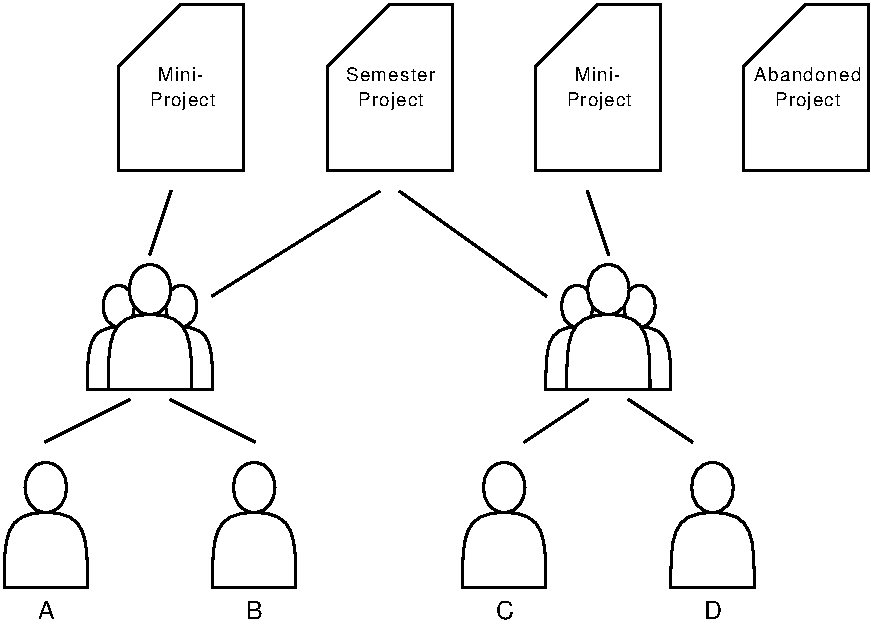
\includegraphics[width=\textwidth]{images/groupprojectdivision.pdf}
                \morscaption{Divided}
                \label{fig:divProjGroup:div}
        \end{subfigure}%
				\hspace{5mm}
        \begin{subfigure}[b]{0.8\textwidth}
                \centering
                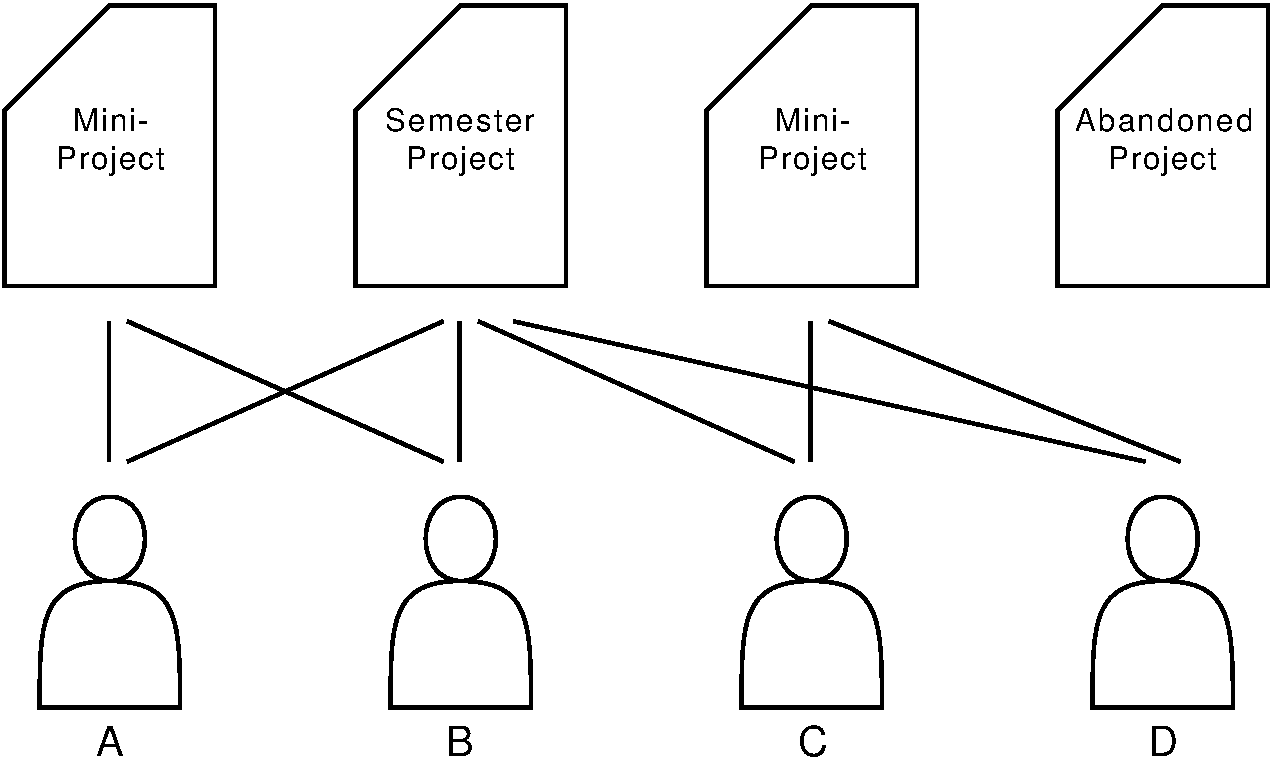
\includegraphics[width=\textwidth]{images/groupprojectunited.pdf}
                \morscaption{United}
                \label{fig:divProjGroup:united}
        \end{subfigure}%
\morscaption{The difference between the two approaches to the division of project and group. Both illustrations use the following example: Students A, B, C, and D collaborate on a semester project, students A and B are working on a mini project, students C and D are working on another mini project, and there exists an abandoned}%
\label{fig:divProjGroup}%
\end{figure}

The differences between these variants are illustrated in \figref{fig:divProjGroup}.
Intuitively the option to divide groups and projects might seem more appropriate since it introduces another level of indirection.
However our interview with Lene W. Even (seen in \appref{sec:lene}) shows that the administrative personnel does not see any benefit from having any extra levels of indirection between students and projects.
%To select which of these divisions to choose we have contacted Lene W. Even and conducted an interview (seen in \appref{sec:lene}).
Since we are working agile we prefer to take the simplest approach, assuming it is viable, and allow for extension of the system later.
We choose to implement groups and projects as one in accordance with our end users' needs and to simplify our system.
% -- note that we have not been in contacts with students for this decision.


%%%%%%%%%%%%%%%%%%%%%%%%%%%%%%%%%%%%%%%%%%%%%%%%%%%%%%%%%%%%%%%%%%%%%%%%%%%%%%%%%%%%%%%%%%%%%%%%%%%%%%%%%%
%%%%%%%%%%%%%%%%%%%%%%%%%%%%%%%%%%%%%%%%%%%%%% COMMENT %%%%%%%%%%%%%%%%%%%%%%%%%%%%%%%%%%%%%%%%%%%%%%%%%%%
%%%%%%%%%%%%%%%%%%%%%%%%%%%%%%%%%%%%%%%%%%%%%%%%%%%%%%%%%%%%%%%%%%%%%%%%%%%%%%%%%%%%%%%%%%%%%%%%%%%%%%%%%%

%Now that the fundamental design is decided, we are able to consider the different types of project group rooms and their properties.


\begin{comment}


\subsection{Recursive tree structure}
Regardless of the group and project relation the structure of project group room rather simple. 
Litmos's groups have a recursive tree structure. 
Project groups can be extended such that a project group can consist of other groups. 
An example of this is at the Software Engineering 6\ths{} semester. 
The students are divided into two main projects. Each of these contains project groups. 

\subsection{Navigation}
\label{sub:designprojectgroupnavigation}
There is currently a problem in Moodle when it comes to navigation. 
When a user is enrolled in a large number of courses their entire front page is filled with links to those courses.
There is no built-in functionality to move or sort the links.
ELSA mentioned this problem during the meeting that we conducted with them described in \secref{sub:elsaInterview}.
%ref Lene
\todo{insert refs to interview with Lene. Hvorfor til Lene når det er ELSA der omtales?}

We want to avoid this problem when we design the navigation for project groups.
Moodle has a navigation block with a list of important links.
We want to add an item to this list that, when expanded, shows the project groups the user is a member of.
Since a supervisor or an administrator might be a member of a many project groups, we want to limit the size of the list of project groups.
We do this by showing at max a preset value, and if the user is a member of more groups we show a link to a page that has a list of all the users's group.


%%%design

%What attribtes should it have
%Aalborg university does not distinguesh between project and groups \ref{sec:lene}

\end{comment}